\documentclass[utf8]{beamer}
\mode<presentation>
\usepackage{listings}
\usepackage{helvet}
\usetheme{Warsaw}
\usecolortheme{whale}
\usefonttheme[onlylarge]{structuresmallcapsserif}
\usefonttheme[onlysmall]{structurebold}

\setbeamercovered{dynamic}
\setbeameroption{show notes}

\begin{document}
\title{Scaling Erlang Web Applications}
\subtitle{100 to 100K users at one web server}
\author{Fernando Benavides (\textit{@elbrujohalcon})}
\institute{Inaka Labs}
\date{\today}
\logo{
\includegraphics[height=0.5cm]{img/inaka_leaf_logo.png}}

\lstset{% general command to set parameter(s)
		basicstyle=\ttfamily\tiny, % print whole listing small
		keywordstyle=\color{black}\bfseries,
		identifierstyle=, % nothing happens
		stringstyle=\ttfamily, % typewriter type for strings
		showstringspaces=false} % no special string spaces

\frame{\titlepage} 

\begin{frame}[t]
	\frametitle{Hello World!}
	\begin{itemize}
		\item<+-> I'm a developer since I was 10
		\item<+-> I'm an Erlang developer since 2008
		\item<+-> I've worked in many dynamic web sites
		\item<+-> Most of them with high scale requirements
		\item<+-> I'll share my experience with you 
	\end{itemize}
	\only<1>{
		\begin{center}
			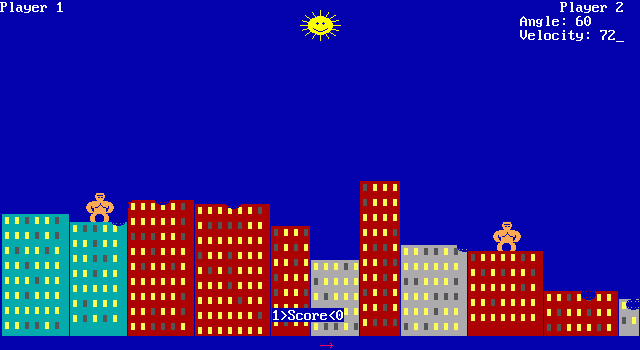
\includegraphics[width=.65\textwidth]{img/Gorillas.png}
		\end{center}
	}
	\only<2>{
		\begin{center}
			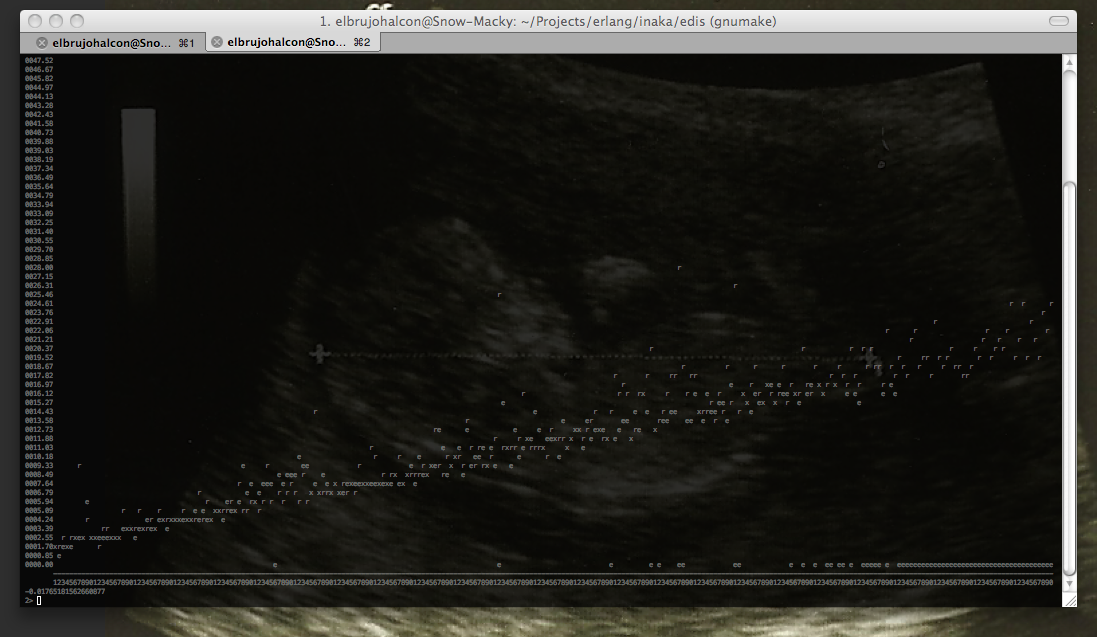
\includegraphics[width=.65\textwidth]{img/ErlangASCIIArt.png}
		\end{center}
	}
	\only<5>{
		\begin{center}
			
\includegraphics[width=.6\textwidth]{img/ShareButton.png}
		\end{center}
	}
\end{frame}

% \frame{\frametitle{Outline}\tableofcontents[pausesections]}
\begin{frame}{Outline}
	\begin{description}
		\item<+->[The Challenge] {\ \\ What do we have to deal with? \\ \ }
		\item<+->[The Plan] {\ \\ How do we face it? \\ \  }
		\item<+->[The Tips and Tricks] {\ \\ What have we learned from it? \\ \ }
	\end{description}
\end{frame}

\section{The Challenge}
\subsection{Description}
\begin{frame}
	We will work on the scalability of a \emph{web} project \pause that has an \emph{HTTP API} \pause and keeps clients \emph{connected} to the server \pause for \emph{long periods} of time.\\
\pause Examples:
	\begin{itemize}
		\item Social sites
		\item Chat sites
		\item Sports sites
	\end{itemize}
\end{frame}

\subsection{Scope}
\begin{frame}
	\emph{We will focus on}
	\begin{itemize}
		\item OTP behaviours
		\item TCP connections
		\item mochiweb
		\item Underlaying system configurations
	\end{itemize}
	\pause
	\emph{We will \textbf{not} deal with}
	\begin{itemize}
		\item Multiple machines/nodes
		\item Databases
	\end{itemize}
\end{frame}

\section{The Plan}
\begin{frame}{The Plan}
	\begin{center}
		
\includegraphics[width=.65\textwidth]{img/challengeaccepted.jpg}
	\end{center}
\end{frame}

\begin{frame}{General Considerations}
	\begin{itemize}
		\item<1,5> Build a system that \alert{works}
		\item<2,5> Automate your clients
		\item<3,5> Keep a human watching
		\item<4,5> Be patient
	\end{itemize}
\end{frame}

\subsection{Finding The Initial Boundaries}
\begin{frame}{Stage 1}{Finding The Initial Boundaries}
	\textsc{Goals}
	\begin{itemize}
		\item Test the system as it is
		\item How many users can the system handle \alert{as is}?
		\item Find $N$ and $C$
	\end{itemize}
\end{frame}
\begin{frame}{Stage 1}{Finding The Initial Boundaries}
	\textsc{Steps}
	\begin{itemize}
		\item Choose $N$ and $C$
		\item Test the API
		\item Test long-lived connections
		\item Test both
		\pause
		\item Repeat with higher values for $N$ and $C$
	\end{itemize}
\end{frame}

\subsection{Blackbox Tests}
\begin{frame}{Stage 2}{Blackbox Tests}
	\textsc{Goals}
	\begin{itemize}
		\item Improve the system environment
		\item Tune-In the machine(s)
		\item \alert{Don't} touch the code
	\end{itemize}
\end{frame}
\begin{frame}{Stage 2}{Blackbox Tests}
	\textsc{Steps}
	\begin{itemize}
		\item Check kernel variables
		\item Check system limits
		\item Check Erlang VM parameters
		\pause
		\item Repeat Stage 1
	\end{itemize}
\end{frame}

\subsection{Erlang Tuning}
\begin{frame}{Stage 3}{Erlang Tuning}
	\textsc{Goals}
	\begin{itemize}
		\item Tune up \alert{your} system
		\item Discover scalability issues and fix them
		\item Find the biggest $N$ and $C$ for \alert{one node}
	\end{itemize}
\end{frame}
\begin{frame}{Stage 3}{Erlang Tuning}
	\textsc{Steps}
	\begin{itemize}
		\item Choose $N$ and $C$ to fail
		\item Find a problem
		\item Fix it
		\item Add it to the list of \emph{Tips and Tricks}
		\pause
		\item Repeat with higher values for $N$ and $C$
	\end{itemize}
\end{frame}

\subsection{Adding Nodes}
\begin{frame}{Stage 4}{Adding Nodes}
	\textsc{Goals}
	\begin{itemize}
		\item Get the system ready to work on many nodes
		\item Design the system topology
		\item Find $N$ and $C$ \alert{per node}
	\end{itemize}
\end{frame}
\begin{frame}{Stage 4}{Adding Nodes}
	\textsc{Steps}
	\begin{itemize}
		\item Get the second node running
		\item Choose $N$ and $C$
		\item Try interconnected instances
		\item Try independent instances
		\pause
		\item Repeat with higher values for $N$ and $C$
	\end{itemize}
\end{frame}

\section{Tips and Tricks}
\begin{frame}{Tips and Tricks}
	\begin{center}
		
\includegraphics[width=.65\textwidth]{img/macgyver.jpg}
	\end{center}
\end{frame}

\subsection{TCP Tunning}

\lstset{language=sh}
\defverbatim[colored]\kernelvars{%
\begin{lstlisting}[frame=single, emph={sysctl}, emphstyle={\color{blue}}]
      sysctl -w net.ipv4.ip_local_port_range="1024 65535"
      sysctl -w net.core.rmem_max=16777216
      sysctl -w net.core.wmem_max=16777216
      sysctl -w net.ipv4.tcp_rmem="4096 87380 16777216"
      sysctl -w net.ipv4.tcp_wmem="4096 65536 16777216"
      sysctl -w net.ipv4.tcp_syncookies=1
      sysctl -w net.ipv4.tcp_mem="50576   64768   98152"
      sysctl -w net.core.netdev_max_backlog=2500
      sysctl -w net.netfilter.nf_conntrack_max=1233000
\end{lstlisting}
}
\defverbatim[colored]\ulimit{%
\begin{lstlisting}[frame=single]
      ulimit -n 999999
\end{lstlisting}
}
\lstset{language=erlang}
\defverbatim[colored]\startchild{%
\begin{lstlisting}[frame=single]
      supervisor:start_child(
      	list_to_atom("module-name_" ++
				integer_to_list(random:uniform(#ofSupervisors))).
\end{lstlisting}
}

\begin{frame}{OS tweaks}
	\emph{Kernel Variables}
	\kernelvars
	\pause
	\only<2>{
		\begin{center}
			
\includegraphics[width=.5\textwidth]{img/omg.jpg}
		\end{center}
	}
	\pause
	\emph{Open Files Limit}
	\ulimit
	\pause
	\emph{Erlang VM tweaks}
	\begin{description}
		\item[+P] Number of Processes
		\item[+K] Kernell Polling
		\item[-smp] SMP Support
	\end{description}
\end{frame}
\begin{frame}{Connection tweaks}
	\begin{description}
		\item<+->[Backlog]\ \\
			\begin{itemize}
				\item Allow more concurrent connections
				\item Remember HTTP \emph{runs on} TCP
			\end{itemize}
		\item<+->[Connections]\ \\
			\begin{itemize}
				\item Don't use just one of them
				\item Check inbound and outbound connections
			\end{itemize}
	\end{description}
\end{frame}
\subsection{OTP}
\begin{frame}{gen\textunderscore event}
	\begin{description}
		\item<+->[sup\textunderscore handler]\ \\
			\begin{itemize}
				\item Don't use it
				\item Monitor the processes instead
			\end{itemize}
		\item<+->[Long Delivery Queues]\ \\
			\begin{itemize}
				\item Use \emph{repeaters}
			\end{itemize}
	\end{description}
\end{frame}
\begin{frame}{gen\textunderscore servers}
	\begin{description}
		\item<+->[Call Timeouts]\ \\
			Remember \texttt{gen\textunderscore server:reply/2}
		\item<+->[Memory Footprint]\ \\
			Remember \texttt{hibernate}
		\item<+->[Long \texttt{init/1}]\ \\
			Use $0$ timeout
	\end{description}
\end{frame}
\begin{frame}{supervisors}
	\begin{itemize}
		\item Sometimes \texttt{simple\textunderscore one\textunderscore for\textunderscore one} supervisors get \alert{overburdened} because they have too many children
		\item Try a supervisor hierarchy with several managers below the main supervisor
		\item Turn \texttt{supervisor:start\textunderscore child/2} calls into something like
		\startchild
	\end{itemize}
\end{frame}
\subsection{Other Stuff}
\begin{frame}
	\begin{description}
		\item<+->[Timers]\ \\
			\begin{itemize}
				\item Don't use the \texttt{timer} module
				\item Use \texttt{erlang:send\textunderscore after}
			\end{itemize}
		\item<+->[Logging]\ \\
			\begin{itemize}
				\item Don't log too much
				\item Use a good logging system
			\end{itemize}
		\item<+->[Registration]\ \\
			\begin{itemize}
				\item Sometimes it's better to register processes instead of keeping track of their pids manually
				\item You can always register processes \alert{both} locally and globally
			\end{itemize}
	\end{description}
\end{frame}

\section{Final Words}
\subsection{Summary}
\begin{frame}{Summary}
	\begin{itemize}
		\item<+-> It is an \alert{iterative} process
		\item<+-> It worked awesomely for us in both experimental and real-life systems
		\item<+-> It's no \alert{silver bullet}
		\item<+-> The list of \emph{Tips and Tricks} grows \alert{constantly} over time
	\end{itemize}
\end{frame}
\subsection{Other stuff}
\begin{frame}{Other stuff}{that we left out of this presentation}
	\begin{itemize}
		\item Adding nodes
		\item Choosing databases
		\item System specific improvements
		\item Measuring tools
	\end{itemize}
\end{frame}
\subsection{Questions}
\begin{frame}{Questions}
	\begin{center}
		
\includegraphics[width=\textwidth]{img/theriddler.jpg}
	\end{center}
\end{frame}

\appendix

\begin{frame}
	\begin{center}
		{\Huge Thanks!}
	\end{center}
\end{frame}

\end{document}